

In this section two optimal control problems involving the overdamped equations are discussed briefly. The differences to the standard optimal control problem, considered in the previous section, are that a non-constant flux is considered instead of a no-flux boundary condition and that observations are made on a subdomain $\Sigma_{Ob}$ or on parts of the boundary, instead of the whole space-time domain $\Sigma$. For illustration, the control is only applied linearly through a source term. 
\begin{figure}[h]
	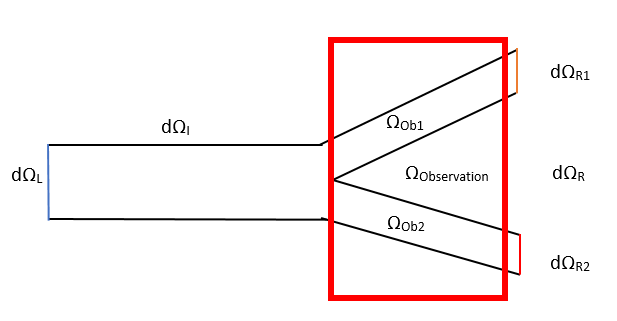
\includegraphics[scale=0.8]{observation.png}
	\caption{Domain of Interest}
	\label{Observation1}
\end{figure}
The first problem of interest is of the form:
\begin{align*}
&\min_{\Sta, w} \quad \frac{1}{2}|| \Sta -\widehat \Sta||^2_{L_2( \Sigma_{Ob})} + \frac{\beta}{2}||w||^2_{L_2(\Sigma)}\\
\text{subject to:}\\
&\partial_t \rho = \nabla^2 \rho - \nabla \cdot (\rho \mathbf{w}) +\nabla \cdot (\rho \nabla V_{ext}) + \nabla \cdot \int_\Omega \rho(r) \rho(r') \nabla V_2(|r-r'|) dr' + w \quad  \quad\text{in} \quad \Sigma,\notag\\
& \rho = \rho_0 \quad \text{at} \quad t=0 \notag\\
& - \mathbf{j} \cdot \nor = \mathbbm{1}_{\partial \Omega_L}( C_{L1}  + C_{L2}\Sta) +\mathbbm{1}_{\partial \Omega_R} ( C_{R1}  + C_{R2}\Sta) +\mathbbm{1}_{\partial \Omega_I} 0, \quad  \quad\text{on} \quad \partial \Omega, 
\end{align*}
where $C_{L1}, C_{L2}, C_{R1}$, $C_{R2}$ are constants and $\mathbbm{1}$ is the indicator function of the set of interest. Considering Figure \ref{Observation1}, the stated non-constant flux boundary condition provides the option of describing a non-constant inflow on boundary $\partial \Omega_L$ and a non-constant outflow on $\partial \Omega_R$, while keeping a no flux condition on the rest of the boundary, denoted by $\partial \Omega_I$.
Furthermore, $\mathbf{j}$ satisfies:
\begin{align*}
\mathbf{j}=\nabla \rho - (\rho \mathbf{w}) +(\rho \nabla V_{ext}) +  \int_\Omega \rho(r) \rho(r') \nabla V_2(|r-r'|) dr'.
\end{align*}
Moreover, let $\widehat \Sta$ be defined such that:
\begin{align*}
\widehat \Sta = \mathbbm{1}_{ \Omega_{Ob1}} \tilde \Sta  +\mathbbm{1}_{ \Omega_{Ob2}} 0.
\end{align*}
This describes a desired state where the particle mass accumulates in the observation domain $\Omega_{Ob1}$ and no particles are found in $\Omega_{Ob1}$. Since observations are only taken on $\Omega_{Ob}$, there is no prescribed desired state on $\Omega / \Omega_{Ob}$.\\
The Lagrangian is of the form:
\begin{align*}
\mathcal{L}(\Sta,w,\Adjb,\Adjc ) &=\frac{1}{2} \int_0^T \int_{\Omega_{Ob}} (\Sta - \widehat \Sta)^2 dr dt + \frac{\beta}{2}\int_0^T \int_\Omega w^2 drdt \\
&+ \int_0^T \int_\Omega \bigg( \partial_t \rho - \nabla^2 \rho + \nabla \cdot (\rho \mathbf{w}) -\nabla \cdot (\rho \nabla V_{ext}) + \nabla \cdot \int_\Omega \rho(r) \rho(r') \nabla V_2(|r-r'|) -w \bigg) \Adjb dr dt\\
&+ \int_0^T \int_{\partial \Omega} \bigg(  \bigg(-\nabla \rho+ (\rho \mathbf{w}) -(\rho \nabla V_{ext}) -  \int_\Omega \rho(r) \rho(r') \nabla V_2(|r-r'|) dr' \bigg)\cdot \nor\\
&  -\mathbbm{1}_{\partial \Omega_L}( C_{L1}  + C_{L2}\Sta) -\mathbbm{1}_{\partial \Omega_R} ( C_{R1}  + C_{R2}\Sta) -\mathbbm{1}_{\partial \Omega_I} 0 \bigg) \Adjc dr dt.
\end{align*}
The derivative of $\mathcal{L}$ with respect to $\rho$ is, as taken from the extended project:
\begin{align*}
&\mathcal{L}_\rho (\rho,{w},\Adjb,\Adjc)h=
\int_\Omega h(T) \Adjb(T) dr\\
&+ \int_0^T \int_\Omega \bigg( \mathbbm{1}_{ \Omega_{Ob}} (\rho- \widehat{\rho})  - \partial_t \Adjb  - \nabla \Adjb \cdot \mathbf{w}  - \nabla^2 \Adjb \notag 
+  \nabla \Adjb \cdot \nabla V_{ext}  \notag \\
&+ \int_\Omega (\nabla  \Adjb(r)+\nabla  \Adjb(r')) \rho(r') \nabla V_2(|r-r'|) dr'+ \int_{\partial \Omega} ( \Adjc(r') - \Adjb(r')) \rho(r')   \frac{\partial V_2(|r-r'|)}{\partial n} dr' \bigg) h dr dt \\
&+  \int_0^T\int_{\partial \Omega}  \bigg(
\bigg(\frac{\partial \Adjb }{\partial n} + \Adjb  \mathbf{w} \cdot \mathbf{n} - \Adjc \mathbf{w} \cdot \mathbf{n}  +  \Adjc \dfrac{\partial V_{ext}}{\partial n} - \Adjb \frac{\partial V_{ext}}{\partial n} + ( \Adjc - \Adjb)  \int_\Omega \rho(r') \frac{\partial V_2(|r-r'|)}{\partial n} dr'\\
& -\mathbbm{1}_{\partial \Omega_L} C_{L2} \Adjc   -\mathbbm{1}_{\partial \Omega_R} C_{R2} \Adjc \bigg)h + \bigg( \Adjc- \Adjb \bigg) \frac{\partial h}{\partial n} \bigg) dr dt =0.
\end{align*}
Then, from appropriate analysis we find that:
\begin{align*}
\Adjc = \Adjb,
\end{align*}
and therefore we get:
\begin{align*}
\mathbbm{1}_{\Omega_{Ob}}(\rho- \widehat{\rho})   - \partial_t  \Adjb  - \nabla \Adjb \cdot \mathbf{w}  - \nabla^2 \Adjb \notag 
+  \nabla \Adjb \cdot \nabla V_{ext}  \notag \\
+ \int_\Omega (\nabla  \Adjb(r)+\nabla  \Adjb(r')) \rho(r') \nabla V_2(|r-r'|) dr' &=0, \quad \text{in} \quad \Sigma, \\
\frac{\partial \Adjb }{\partial n}  -\mathbbm{1}_{\partial \Omega_L} C_{L2} \Adjb   -\mathbbm{1}_{\partial \Omega_R} C_{R2} \Adjb&=0, \quad \text{on} \quad \partial \Omega.
\end{align*}
In particular, this is:
\begin{align*}
\mathbbm{1}_{\Omega_{Ob1}}(\rho- \widehat{\rho}) +\mathbbm{1}_{\Omega_{Ob2}}\rho  - \partial_t  \Adjb  - \nabla \Adjb \cdot \mathbf{w}  - \nabla^2 \Adjb \notag 
+  \nabla \Adjb \cdot \nabla V_{ext}  \notag \\
+ \int_\Omega (\nabla  \Adjb(r)+\nabla  \Adjb(r')) \rho(r') \nabla V_2(|r-r'|) dr' &=0, \quad \text{in} \quad \Sigma, \\
\frac{\partial \Adjb }{\partial n}  -\mathbbm{1}_{\partial \Omega_L} C_{L2} \Adjb   -\mathbbm{1}_{\partial \Omega_R} C_{R2} \Adjb&=0, \quad \text{on} \quad \partial \Omega.
\end{align*}
The gradient equation is:
\begin{align*}
w = \frac{1}{\beta}\Adjb.
\end{align*}
Comparing this to the previous section, it can be observed that the gradient equations have opposite signs. This is due to the different construction of the Lagrangian. (+++ I really don't want to change this. Let's see! +++)


